\begin{table*}[t]
\centering\small
\adjustbox{max width=\textwidth}{\begin{tabular}{l c ccccccc}
\toprule
Decoder & R$^2_{\mathrm{vw}}$ & \texttt{tx} & \texttt{ty} & \texttt{tz} & \texttt{rx} & \texttt{g1} & \texttt{g2} & \texttt{g3} \\
\midrule
Wiener filter, global norm. & 0.319 & 0.17 & 0.02 & 0.15 & 0.34 & 0.42 & 0.32 & 0.25 \\
Wiener filter & 0.321 & 0.18 & 0.03 & 0.17 & 0.34 & 0.42 & 0.33 & 0.25 \\
Kalman filter & 0.242 & 0.17 & 0.08 & 0.18 & 0.33 & 0.35 & 0.23 & 0.13 \\
GRU & 0.626{\scriptsize$\pm$0.002} & 0.30 & 0.25 & 0.32 & 0.51 & 0.74 & 0.65 & 0.56 \\
Causal Transformer & 0.578 & 0.31 & 0.26 & 0.34 & 0.54 & 0.72 & 0.55 & 0.49 \\
Multi-day GRU, no aug. & 0.559 & 0.20 & 0.04 & 0.30 & 0.38 & 0.74 & 0.57 & 0.48 \\
\textbf{Multi-day GRU (ours)} & 0.574{\scriptsize$\pm$0.000} & 0.20 & 0.07 & 0.24 & 0.39 & 0.73 & 0.58 & 0.53 \\
\bottomrule
\end{tabular}
}
\caption{Within-session decoding on FALCON H1 held-in minival blocks (13 blocks, 6 days). R$^2_{\mathrm{vw}}$ is FALCON's variance-weighted R$^2$, averaged over blocks ($\pm$: std over seeds; 2 seeds for GRU and multi-day GRU). Per-DoF columns give R$^2$ pooled over blocks. For reference, FALCON reports held-in R$^2$ on its private test split of 0.24 (Wiener filter), 0.51 (RNN) and 0.68 (NDT2 Multi)~\cite{karpowicz2024falcon}; those values are not directly comparable to ours.}
\label{tab:within}
\end{table*}

\paragraph{Within session.}
\begin{itemize}
\item \textbf{Recurrent models dominate linear decoders} (Table~\ref{tab:within}, Fig.~\ref{fig:within}). The GRU reaches R$^2$=\GRUWithin{}, against \WienerWithin{} for the Wiener filter and \KalmanWithin{} for the Kalman filter.
\item \textbf{Per-DoF pattern.} The pooled per-DoF R$^2$ shows the same pattern for every decoder: grasp dimensions and wrist roll are decoded far better than translation, and $t_y$ is the hardest. The FALCON metric is variance-weighted, so it is dominated by the well-decoded grasp dimensions; a decoder that is good on the metric can still be poor at moving the hand in space. This is one reason we put the robot's assistance on translation and alignment.
\item \textbf{Multi-day GRU} (R$^2$=\MSGRUWithin): per-day read-ins slightly \emph{hurt} within-session accuracy relative to a single shared read-in. The extra $6\times$ input parameters overfit 2{,}300\,s of training data; its training loss ended well below the GRU's while its validation loss stayed higher.
\end{itemize}

\begin{figure*}[t]
\centering
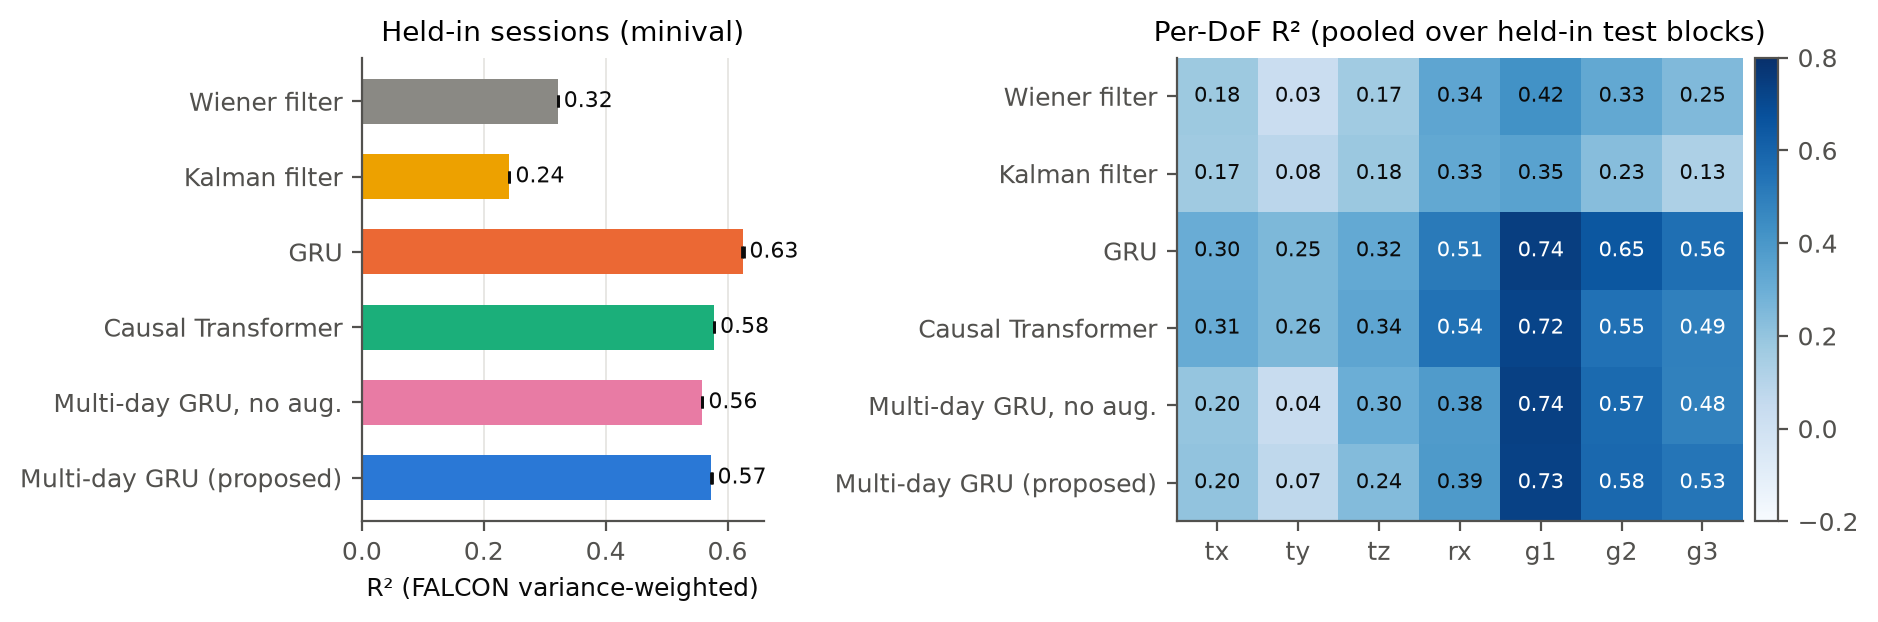
\includegraphics[width=0.9\textwidth]{figures/decoding_within.png}
\caption{Held-in decoding: variance-weighted R$^2$ (left) and per-DoF R$^2$ (right).}
\label{fig:within}
\end{figure*}

\begin{table*}[t]
\centering\small
\adjustbox{max width=\textwidth}{\begin{tabular}{l c ccc}
\toprule
& zero-shot & 10\,s & 20\,s & 45\,s \\
\midrule
Wiener filter, global norm. & 0.048 & -- & -- & -- \\
Wiener filter, held-in + new & 0.110 & 0.115 & 0.116 & 0.122 \\
Wiener filter, new data only & -- & -0.121 & 0.002 & 0.035 \\
Kalman filter & 0.039 & -- & -- & -- \\
GRU, fine-tune all & 0.247{\scriptsize$\pm$0.022} & 0.116{\scriptsize$\pm$0.006} & 0.160{\scriptsize$\pm$0.023} & 0.238{\scriptsize$\pm$0.047} \\
Causal Transformer, fine-tune all & 0.286 & 0.079 & 0.189 & 0.265 \\
Multi-day GRU, fine-tune all & 0.107{\scriptsize$\pm$0.078} & 0.217 & 0.198 & 0.222 \\
Multi-day GRU no aug., new read-in & 0.227 & 0.277 & 0.294 & 0.271 \\
\textbf{Multi-day GRU, new read-in (ours)} & 0.107{\scriptsize$\pm$0.078} & 0.272{\scriptsize$\pm$0.053} & 0.266{\scriptsize$\pm$0.049} & 0.285{\scriptsize$\pm$0.036} \\
\bottomrule
\end{tabular}
}
\caption{Cross-session decoding: R$^2_{\mathrm{vw}}$ on 7 later days (6--20 days after training), tested on block~B. Columns give the labelled seconds of the same day's block~A used for recalibration. All rows normalise inputs per day from block~A without labels, except ``global norm.'' This is our protocol, not FALCON's private split.}
\label{tab:cross}
\end{table*}

\paragraph{Across days.} Every decoder degrades on later days (Table~\ref{tab:cross}, Fig.~\ref{fig:cross}).
\begin{itemize}
\item \textbf{Normalisation.} Per-day z-scoring from unlabelled data is itself worth about 0.06 R$^2$ for the Wiener filter (\WienerZS{} vs \WienerGlobalZS{} with global normalisation).
\item \textbf{Zero-shot.} Neural decoders transfer better than linear ones. The single-read-in causal Transformer (0.286) and GRU (0.247) are the best zero-shot decoders. The multi-day GRU with an \emph{averaged} read-in is poor and unstable across seeds (\MSGRUZS$\pm$0.078), because the mean of day-specific read-ins is not itself a trained read-in.
\item \textbf{Full fine-tuning on seconds of data is harmful.} The GRU and the Transformer fine-tuned end-to-end on 10\,s fall far \emph{below} their own zero-shot accuracy (0.116 and 0.079), and recover only partly at 45\,s. A Wiener filter trained only on the new seconds is near or below zero.
\item \textbf{Read-in-only recalibration is the only adaptation that never hurts.} Fitting only a new input layer for the frozen multi-day core lifts it from \MSGRUZS{} to 0.27 with 10\,s and \MSGRUFew{} with \RecalMax\,s. At every budget this beats every other recalibration strategy: \GRUFew{} for the fine-tuned GRU at \RecalMax\,s, and \WienerPooledFew{} for the refit Wiener filter.
\item \textbf{The honest bottom line.} It does \emph{not} beat the best zero-shot model, the causal Transformer, by a meaningful margin. At this data scale (2{,}300\,s of training data, 6 days) the main benefit of read-in recalibration is robustness, since it never collapses, rather than higher accuracy than a well-regularised zero-shot decoder.
\item \textbf{Augmentation.} Removing the nonstationarity augmentation did not hurt few-shot accuracy here (single seed); we do not claim a benefit from it at this scale.
\end{itemize}
The absolute numbers (R$^2\approx0.2$--0.3 across days) underline how far 7-DoF decoding is from ``solved'' at this data scale, and motivate the shared autonomy below.

\begin{figure*}[t]
\centering
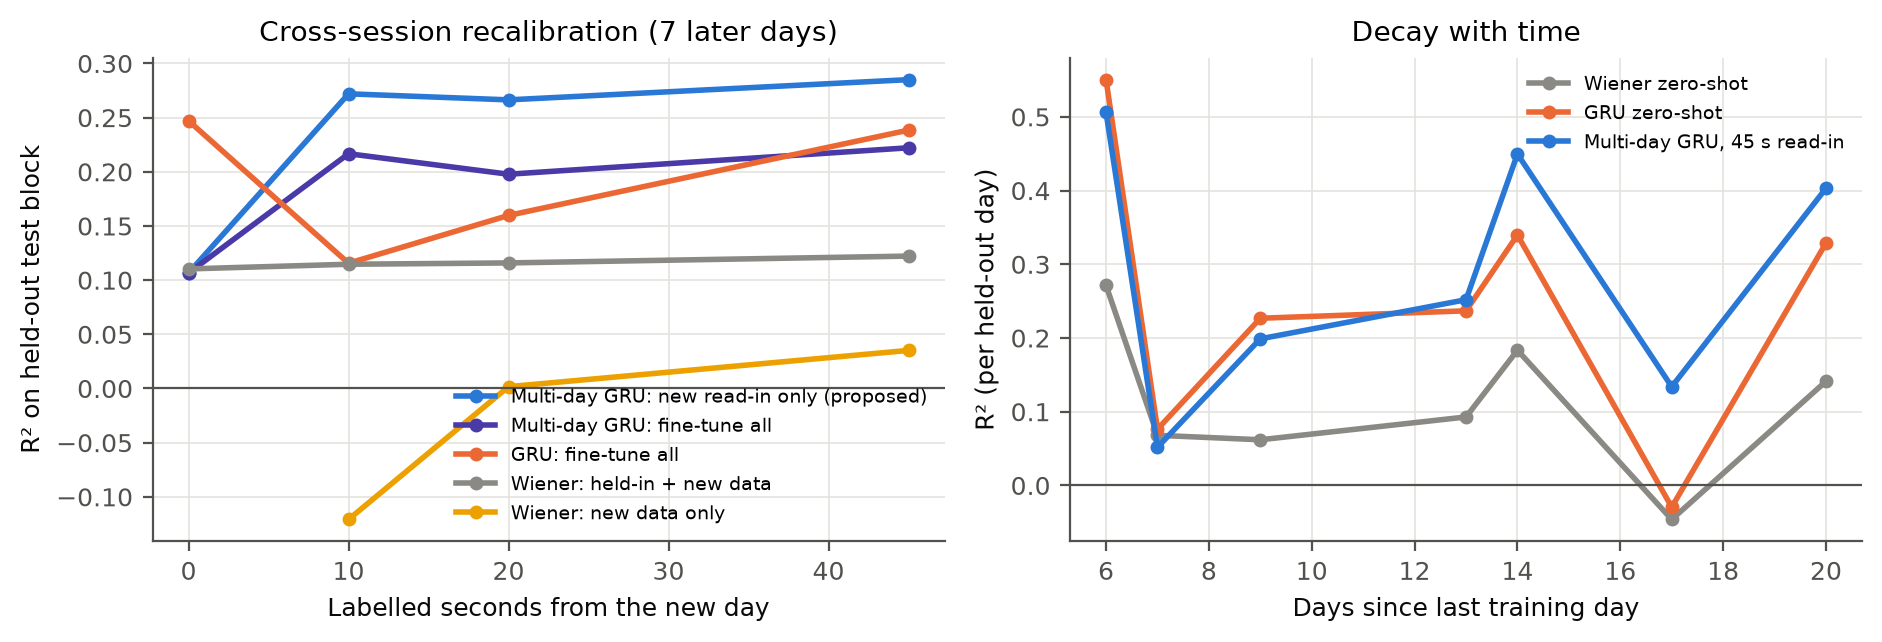
\includegraphics[width=0.9\textwidth]{figures/decoding_cross_session.png}
\caption{Cross-session recalibration (left) and per-day R$^2$ against days since the last training day (right).}
\label{fig:cross}
\end{figure*}

\begin{figure*}[t]
\centering
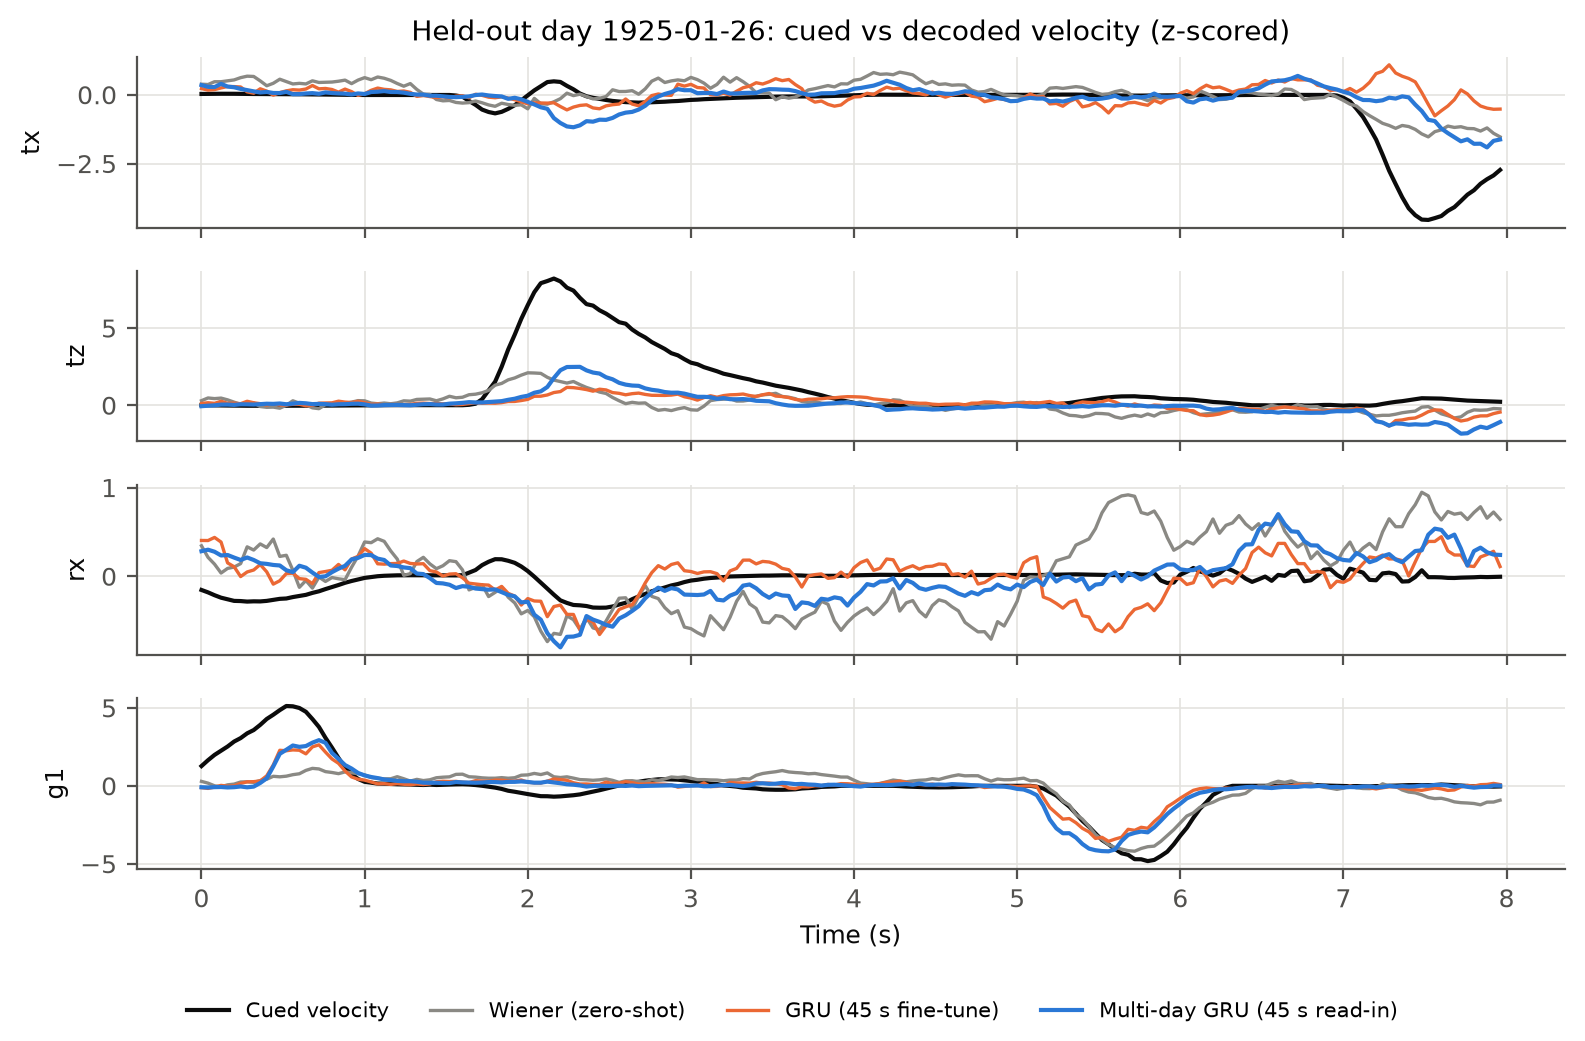
\includegraphics[width=0.8\textwidth]{figures/decoding_traces.png}
\caption{Cued (black) and decoded velocity on a held-out day, in z-scored units, for four of the seven DoF: zero-shot Wiener filter, GRU fine-tuned on 45\,s, and multi-day GRU with a 45\,s read-in. Translation ($t_x$, $t_z$) is decoded far less faithfully than wrist roll and grasp.}
\label{fig:traces}
\end{figure*}
